\documentclass{kththesis}
\usepackage{graphicx}

\usepackage{csquotes} % Recommended by biblatex
\usepackage{biblatex}
\addbibresource{references.bib} % The file containing our references, in BibTeX format

\setlength{\parskip}{1em}
\setlength{\parindent}{0em}


\title{Visualizing Simulated Trajectory Data}
\subtitle{Making simulated pedestrian trajectory data interactive with D3.js}
\alttitle{Titel på svenska}
\author{Christina Sonebo, Joel Ekelöf}
\email{sonebo@kth.se, joeleke@kth.se}
\supervisor{Christopher Peters}
\examiner{Örjan Ekeberg}
\school{School of Electrical Engineering and Computer Science}
\date{\today}


\begin{document}

% Frontmatter includes the titlepage, abstracts and table-of-contents

\titlepage

\begin{abstract}
  English abstract goes here.

\end{abstract}


\begin{otherlanguage}{swedish}
  \begin{abstract}
Svenska abstract
  \end{abstract}
\end{otherlanguage}


\tableofcontents


% Mainmatter is where the actual contents of the thesis goes
\mainmatter


\chapter{Introduction}

\section{Research Question}

\begin{itemize}
    \item How can visualization aid users in their tasks of interpreting and exploring trajectory data?
    \item How can D3.js and other web development tools be used to create such a visualization?
\end{itemize}


\section{Background}


This section will begin by introducing the research area of data visualization and methods of user evaluation. It will then proceed to describe crowd simulations and trajectory data. Lastly it will present concepts that are key to understanding the process of building data visualizations with web development tools.


\subsection{Data Visualization}

Data visualization is the creation of graphical representations or images of information. It can be viewed as an application of computer graphics, using computer graphics methods to display data. But rather than focusing on purely visual aspects, it aims to aid users in discovering and formulating ideas about datasets through visualization \cite{Chad}.

Consequently it is composed of several disciplines such as human-computer interaction, user perception, statistics and data mining - combining computational power with the strengths that human visual perception offers \cite{Chad}.

\subsection{User Perception and Evaluation}

The primary purpose of data visualization systems is to assist users in the exploration and understanding of data. First, it is key to ask how such a system can be designed to be \emph{efficient}. Secondly it is important to ask how efficiency is \emph{measured} and \emph{evaluated}. This section will introduce theories and methods used to answer these questions when designing and evaluating data visualization systems.

\subsubsection{The Visual Information Seeking Mantra}
The Visual Information Seeking mantra - \emph{overview first, zoom and filter, then details-on-demand}, was first described by Schneiderman in 1996 and is widely cited within information visualization research \cite{Craft}. It attempts to describe how data is effectively presented to users and often serves as a guideline and as an inspiration for practitioners within the field data visualization. The mantra consists of five tasks that users of a visualization system should be able to perform:


\begin{itemize}
    \item Overview first: capture the entire dataset in one view.
    \item Zoom and filter: remove unnecessary information and reduce the amount of data displayed.
    \item Details on demand: display additional information if requested, without requiring a change of view.
    \item Relate: enable the users to observe relationships in the data.
    \item History: enable users return to a previous state, and compare it to a other states of representation.
    \item Extract: extract information of interest, so that users do not need to reproduce the same steps of data manipulation to retrieve it again.
\end{itemize}


\subsubsection{Heuristics and Evaluation of Visualizations}

There are several different approaches to evaluate visualization environments. However, after the visual information seeking mantra was introduced - heuristics evaluation has since become the basis for such evaluations \cite{Freitas2014}.

A heuristic evaluation is defined as an inspection of a user interface, where an individual or a group evaluates it according to a list of principles \cite{Wilson20141}. This inspection can be done on a specification, a prototype, or a finished product. When evaluating visualizations, the heuristics is typically a list of tasks for users to perform \cite{Freitas2014}.


As for the tasks and the evaluation of effectiveness, Christopher D. Hundhausen presents three perspectives on this in "Evaluating Visualization Environments: Cognitive, Social, and Cultural Perspectives". In this thesis will use the cognitive perspective, which defines the measurement of a visualization's effectiveness to be be the extent to which it promotes task efficiency \cite{Hundhausen2014}. The aim of the visualization from this perspective is to transform cognitive operations into easier perceptual ones -  resulting in a more efficient human task performance.


% What is trajectory data?
\subsection{Trajectory Data}


A trajectory is the trace of a moving object - a path through space as a function of time.
Examples of moving objects could be anything from vehicles to particles - their commonality being that they are entities with positioning or geometrical properties that change over time \cite{Tradef2}.

The data of trajectories is typically represented by a set of chronologically ordered location points, $ P = \langle x_{n}, y_{n}, t_{n} \rangle $ where $x_{i}, y_{i}$ are geographical coordinates at time $t_{i}$, and \emph{n} is the total number of elements in the series \cite{Tradef1}. When put together, these create a trajectory $ T = \{ P_{1}, P_{2},...,P{n} \} $.

It is also possible that the data contains information besides the location points themselves. These attributes are either derived from or associated with the data and is often referred to as thematic \cite{Ref1}. Examples of such attributes could be category, the speed of an object at a given time, or what direction the object is facing.


%\subsubsection{Anomaly Detection}


%Using VA to create clusters of trajectories
%\subsubsection{Clustering Trajectories}
%use k-means? http://bl.ocks.org/feyderm/75c18a9143aac50a24e392762f10d6a4
%https://bl.ocks.org/wolfDynamics/8682a6ff548e820d4acb5cd0e87ca603
% //www.npmjs.com/package/density-clustering <- packages in js already available for all of the different kinds of clustering.





% What will we conduct research on, how has it been altered (petter har fixat datapunkterna!)
\subsection{The Dataset}

The chosen dataset for this thesis has its origins from the UCY Computer Graphics Lab \cite{Cyprus}. It consists of video of students walking through a campus area and a file containing the series of splines describing their movement.


%It could be interesting to render the not so fixed dataset as well.



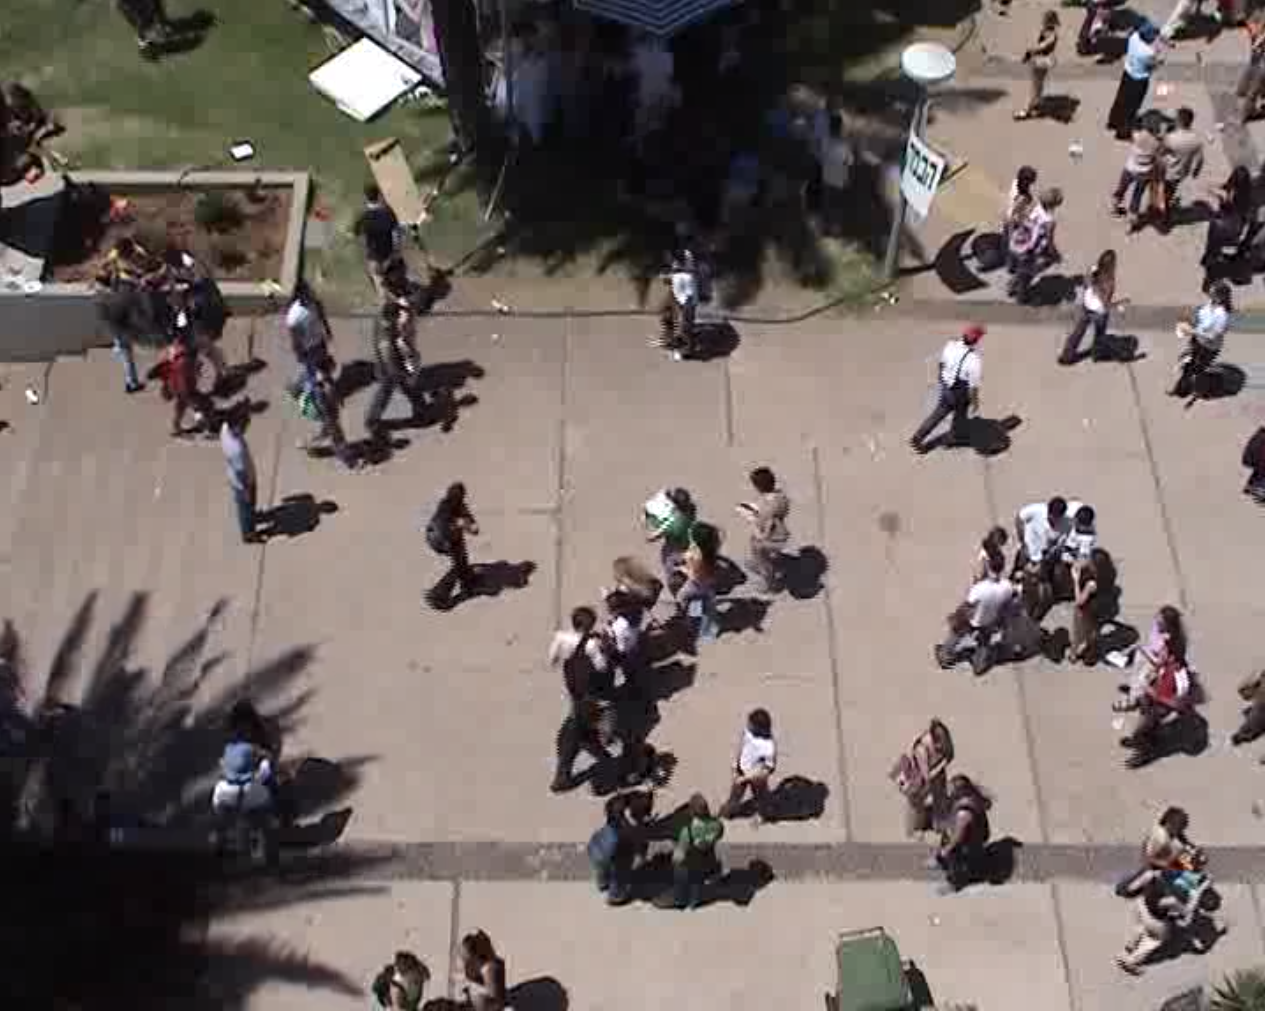
\includegraphics[width= 8.0cm , height= 5.0cm]{images/clip.png}


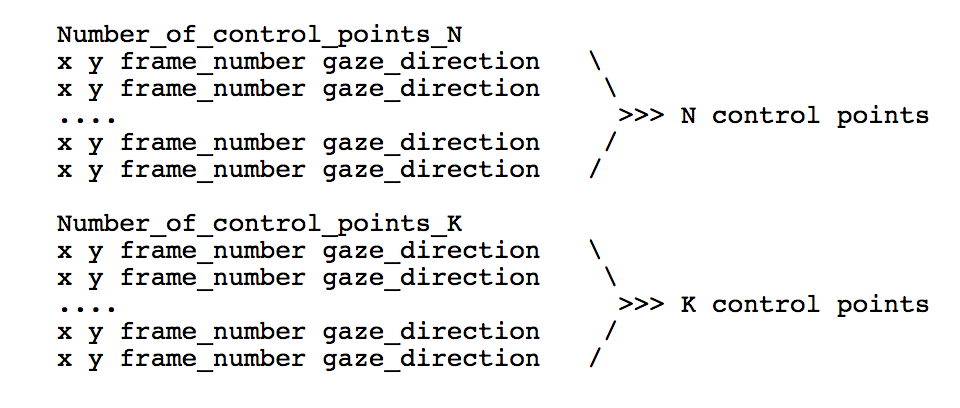
\includegraphics[width= \textwidth]{images/fileformat.png}


\subsection{Tools}

\subsubsection{Browser Architecture}

Browsers consist of several modular pieces, each responsible for certain functionalities:
\begin{itemize}
    \item UI layer - draws the user interface, e.g. windows and buttons.
    \item Rendering engine - parses, tokenizes and renders the HTML.
    \item Network layer - manages network operations needed to retrieve HTML and assets.
    \item JavaScript engine - interprets and executes the JavaScript code.
\end{itemize}

\subsubsection{HTML/CSS}
HTML is an abbreviation for HyperText Markup Language. It consists of elements representing layout and formatting.

\subsubsection{JavaScript}
JavaScript is a programming language that is mainly used to dynamically script webpages through manipulating the DOM. \cite{JS}

The Document Object Model is loaded in the browser and represents the the HTML document as a tree with nodes for each part of the document, such as an element, comment etc. \cite{DOM}
The DOM is one of the most used APIs on the web since it allows code in the browser to interact with any part of the document.

\subsubsection{D3 - Data Driven Documents}
D3 is a JavaScript library dedicated to data visualization. D3 is a data-driven approach to modify the DOM. \cite{D3}

\subsubsection{JSON}

\subsection{Related Work}
 \begin{itemize}
     \item Visual Analytics Tools for Analysis of Movement Data
     \item An Exploratory Spatial Data Analysis (ESDA) Toolkit for the Analysis of Activity/Travel Data
 \end{itemize}


\chapter{Methods}

\section{Tasks and User Analysis}



\subsection{Design}

%what is data visualization and what theories are useful when building a visualization system?
\section{Prototype}

\section{User Evaluation}







\chapter{Results}

\chapter{Discussion}
\section{Future Work}

Considering that this thesis has focused on the three first components of the visualization seeking mantra, we suggest the remaining three - \emph{relate, history and extract} as possible features to extend the current implementation with.

Another thing which might be of interest is clustering, as suggested by Adrienko et al, especially for visualizations of trajectories in the context of crowd simulations as it could act as a tool for anomaly detection. It could bring another dimension to the exploration of the data in terms of relationships that are made discovarble through this kind of data analysis. There have been some implementations such as TRACLUS - but also attempts have been made through discrete methods such as K-Means



\chapter{Conclusion}


\printbibliography[heading=bibintoc] % Print the bibliography (and make it appear in the table of contents)

\appendix



\end{document}


\documentclass{article}
\usepackage[utf8]{inputenc}
\usepackage{graphicx}
\usepackage{biblatex}
\usepackage{url}
\addbibresource{ref.bib}
\setlength{\parskip}{1em}
\setlength{\parindent}{0em}



\usepackage{listings}

\title{Visualization of Trajectory Data}
\author{Christina Sonebo, Joel Ekelöf}
\date{February 2018}

\begin{document}

\maketitle

\begin{abstract}

\end{abstract}

\newpage

\tableofcontents

\newpage


\printbibliography

\end{document}
